\documentclass[11pt]{article}

%%
%% PACKAGES
%%

\usepackage[margin=0.9in, top=0.8in, bottom=1.0in]{geometry}
\usepackage[charter]{mathdesign} % Main font
\usepackage[scaled]{beramono} % Lovely monospace font
\usepackage[T1]{fontenc}
%\usepackage{amsmath, amssymb}
\usepackage{mathtools}
\usepackage{mathdots}
\usepackage{titlesec} % Custom section headings.
\usepackage{microtype}
\usepackage{xcolor}
\usepackage{xspace}
\usepackage{xfrac}
\usepackage{calc}
\usepackage{subcaption}

% Graphics.
%\usepackage{graphicx}
\usepackage[update,prepend]{epstopdf} % To use eps files.

% Code listings.
\usepackage{listings} % Code listings.
\usepackage{matlab-prettifier} % MATLAB code listings

% Tweaks for captions and enumerations.
\usepackage[labelfont=bf]{caption} % Figure captions.
\usepackage{enumitem} % Fine tuning enumerations.
%\usepackage{floatrow} % Captions to the right of figures.

% Plotting and drawing
\usepackage{tikz} % This automatically loads graphicx!
\usetikzlibrary{calc} % For relative positions to defined coords
\usepackage{pgfplots} % Scientific plotting tools
\pgfplotsset{compat=1.7}

% Figure placement
\usepackage{wrapfig}
\captionsetup[wrapfigure]{margin=0.5cm}

% Packages to makes tables pretty.
\usepackage{array}
\usepackage{booktabs}
\setlength{\heavyrulewidth}{1.5pt}
\setlength{\abovetopsep}{4pt}

% Fancyhdr package stuff...
\usepackage{fancyhdr}
\setlength{\headheight}{0pt}
\setlength{\footskip}{50pt}
\renewcommand{\headrulewidth}{0pt}
\renewcommand{\footrulewidth}{0pt}

%%
%% SETTINGS
%%

% Path to look for graphics
\graphicspath{{../images/}}
%\epstopdfsetup{outdir=../images/}

% Caption spacing
\setlength{\abovecaptionskip}{0pt}

% List spacing
\setlist{noitemsep}

% Math operator font
\DeclareSymbolFont{sfoperators}{OT1}{cmss}{m}{n}
\DeclareSymbolFontAlphabet{\mathsf}{sfoperators}
\makeatletter
\def\operator@font{\mathgroup\symsfoperators}
\makeatother

%% No indent all paragraphs
%\setlength{\parindent}{0in}

% Figure references
\newcommand{\figref}[1]{Figure~\ref{#1}}

% Special format section headings
\titleformat{\section}%
	{\large\bf\scshape}% Text formatting
	{\arabic{section}}% Number
	{1em}% Space between number and text
	{}% Code before
	[]% Code after
\titleformat{\subsection}%
	{\normalsize\bf\scshape}% Text formatting
	{\arabic{section}.\arabic{subsection}}% Number
	{1em}% Space between number and text
	{}% Code before
	[]% Code after
%\titleformat{\subsubsection}%
%	{\color{blue}}% Text formatting
%	{\arabic{subsubsection} $\rightarrow$}% Number
%	{1em}% Space between number and text
%	{}% Code before
%	[]% Code after

\definecolor{mygray}{rgb}{0.4, 0.4, 0.4}
\lstset{
style=Matlab-editor,
mlscaleinline=false,
basicstyle=\ttfamily\lst@ifdisplaystyle\scriptsize\fi,
frame=single,
rulecolor=\color{mygray},
numbers=left,
numbersep=10pt,
numberstyle=\footnotesize \ttfamily \color{mygray},
xleftmargin=30pt,
xrightmargin=5pt,
framexleftmargin=4pt,
framextopmargin=2pt
}

% Allow white-space to be eaten within any lst environments between returns.
\lstset{breaklines,breakatwhitespace}

% Define the | chacacter as shorthand for inline listings.
\lstMakeShortInline{`}

%%
%% COMMANDS
%%

% Various plot lines to include in-line.
\newcommand{\solidrule}[1][8mm]{\rule[0.5ex]{#1}{1.5pt}}
\newcommand{\dashrule}{\mbox{%
	\solidrule[2mm]\hspace{1mm}\solidrule[2mm]\hspace{1mm}\solidrule[2mm]}}
\newcommand{\dotdashrule}{\mbox{%
	\solidrule[0.5mm]\hspace{1mm}\solidrule[2mm]\hspace{1mm}\solidrule[0.5mm]\hspace{1mm}\solidrule[2mm]}}

% Automated file inclusion for code listings
\makeatletter
\def\includecode{\@ifnextchar[{\@with}{\@without}}
\def\@with[#1]#2{
}
\def\@without#1{
  \lstinputlisting[caption=\ttfamily\protect\detokenize{#1}, escapechar=, frame=single]{../matlab_code/#1}
}
\makeatother

% Degree symbol.
\newcommand{\degree}{\ensuremath{^\circ}}

% Superscript text: 1st, 2nd, 3rd, 4th
\newcommand{\suptext}[1]{\ensuremath{^\text{#1}}\xspace}
\newcommand{\st}{\suptext{st}}
\newcommand{\nd}{\suptext{nd}}
\newcommand{\rd}{\suptext{rd}}
\let\oldth\th % Reassign the current \th command
\renewcommand{\th}{\suptext{th}}

% Underline matrices
\newcommand{\ul}[1]{\smash{\underline{#1}}}
\newcommand{\uul}[1]{\smash{\underline{\underline{#1}}}}

% Partial derivatives
\newcommand{\pp}[2]{\ensuremath{\frac{\partial#1}{\partial#2}}}

% Math operators
\DeclareMathOperator\erf{erf}
\DeclareMathOperator\var{Var}

% Big O notation
\newcommand{\bigo}{\ensuremath{\mathcal{O}}}

% Text max and min
\newcommand{\tmax}{\ensuremath{\text{max}}}
\newcommand{\tmin}{\ensuremath{\text{min}}}

% Norm
\newcommand{\norm}[1]{\ensuremath{\left| #1 \right|}}

% Expectation
\newcommand{\xpect}[1]{\ensuremath{\left\langle #1 \right\rangle}}

% Bold vectors
% Option 1: Works on more than single tokens, but makes regular letters italic as well as bold.
%\renewcommand{\vec}[1]{\mathbold{#1}}
% Option 2: Only works if a single token is passed to the command, but makes regular letters bold only.
\newcommand{\mb}[1]{
	\ifcat\noexpand#1\relax
		\expandafter\mathbold
	\else
		\expandafter\mathbf
	\fi{{#1}}
}

% Underlines for tensor notation.
\newcommand{\tsr}[1]{\ensuremath{\underline{#1}}}
\newcommand{\tsrr}[1]{\ensuremath{\underline{\underline{#1}}}}


%%
%% DOCUMENT START
%%

\begin{document}


\newcommand{\widesim}[2][1.5]{
  \mathrel{\overset{#2}{\scalebox{#1}[1]{$\sim$}}}
}

\pagestyle{fancyplain}
\lhead{}
\chead{}
\rhead{}
\lfoot{\hrule UQ: Homework 2}
\cfoot{\hrule \thepage}
\rfoot{\hrule Ryan Skinner}

\noindent
{\Large Homework 2}
\hfill
{\large Ryan Skinner}
\\[0.5ex]
{\large ASEN 6519: Uncertainty Quantification}
\hfill
{\large Due 2016/03/08}\\
\hrule
\vspace{6pt}

%%%%%%%%%%%%%%%%%%%%%%%%%%%%%%%%%%%%%%%%%%%%%%%%%
%%%%%%%%%%%%%%%%%%%%%%%%%%%%%%%%%%%%%%%%%%%%%%%%%
\section*{Problem 1} %%%%%%%%%%%%%%%%%%%%%%%%%%%%
%%%%%%%%%%%%%%%%%%%%%%%%%%%%%%%%%%%%%%%%%%%%%%%%%
%%%%%%%%%%%%%%%%%%%%%%%%%%%%%%%%%%%%%%%%%%%%%%%%%

Given the joint CDF of random variables $X_1$ and $X_2$,
\begin{equation}
F_{X_1,X_2}(x_1,x_2) = 1 - \exp(-x_1) - \exp(-x_2) + \exp(-x_1-x_2-x_1x_2)
, \quad x_1,x_2 \ge 0,
\end{equation}
we are tasked with finding the marginal CDF $F_{X_1}(x_1)$ and the conditional CDF $F_{X_2|X_1}(x_2|x_1)$, and subsequently generating realizations of $X_1,X_2$ using the inversion method.

The marginal CDF of $X_1$ is trivially calculated in the limit $x_2 \rightarrow \infty$ as
\begin{equation}
\boxed{F_{X_1}(x_1)} = F_{X_1,X_2}(x_1,\infty) = 1 - \exp(-x_1)
.
\end{equation}

Applying the relation
\begin{equation}
F_{X_2|X_1}(x_2|x_1) = \left( \int_0^{x_2} f_{X_1,X_2}(x_1,t_2) dt_2 \right) \Big/ f_{X_1}(x_1)
,
\end{equation}
where the marginal and joint pdfs are
\begin{align*}
f_{X_1}(x_1) &= \partial_{x_1} F_{X_1}(x_1) \\
f_{X_1,X_2}(x_1,x_2) &= \partial_{x_1} \partial_{x_2} F_{X_1,X_2}(x_1,x_2)
,
\end{align*}
it can be shown that
\begin{equation}
\boxed{F_{X_2|X_1}(x_2|x_1)} = 1 - (1+x_2) \exp(-[1+x_1]x_2)
,
\end{equation}
which is impossible to invert analytically, though computational root-finding methods show success.

Realizations of $X_1,X_2$ are generated in the standard manner: for each $i = 1, ..., N$, a random variable $U_1^i \sim U[0,1]$ is generated, and set equal to $F_{X_1}(x_1)$, which can be solved for realization $x_1^i$. Another random variable $U_2^i \sim U[0,1]$ is generated and set equal to $F_{X_2|X_1}(x_2|x_1)$, which is then solved numerically for $x_2^i$, given $x_1^i$. We choose Matlab's `fzero` function as our root finder.

In \figref{fig:prob1}, we generate $N=10,\!000$ realizations and compare the cumulative expectation of the first $n$ samples to the analytical expectations
\begin{equation}
\begin{aligned}
\langle x_1 \rangle &= 1.0 \\
\langle x_1 \rangle &= 1.0 \\
\langle x_1 x_2 \rangle &= 0.596347
\end{aligned}
\end{equation}
All three quantities approach their analytical values, and the relative error in each quantity is seen to decrease as $n$ increases.

This method of verification is by no means rigorous. The mean square error of the empirical CDF or pdf would be a better way of checking the validity of our answers, but this suffices for the purposes of this exercise.

\begin{figure}[t]
\centering
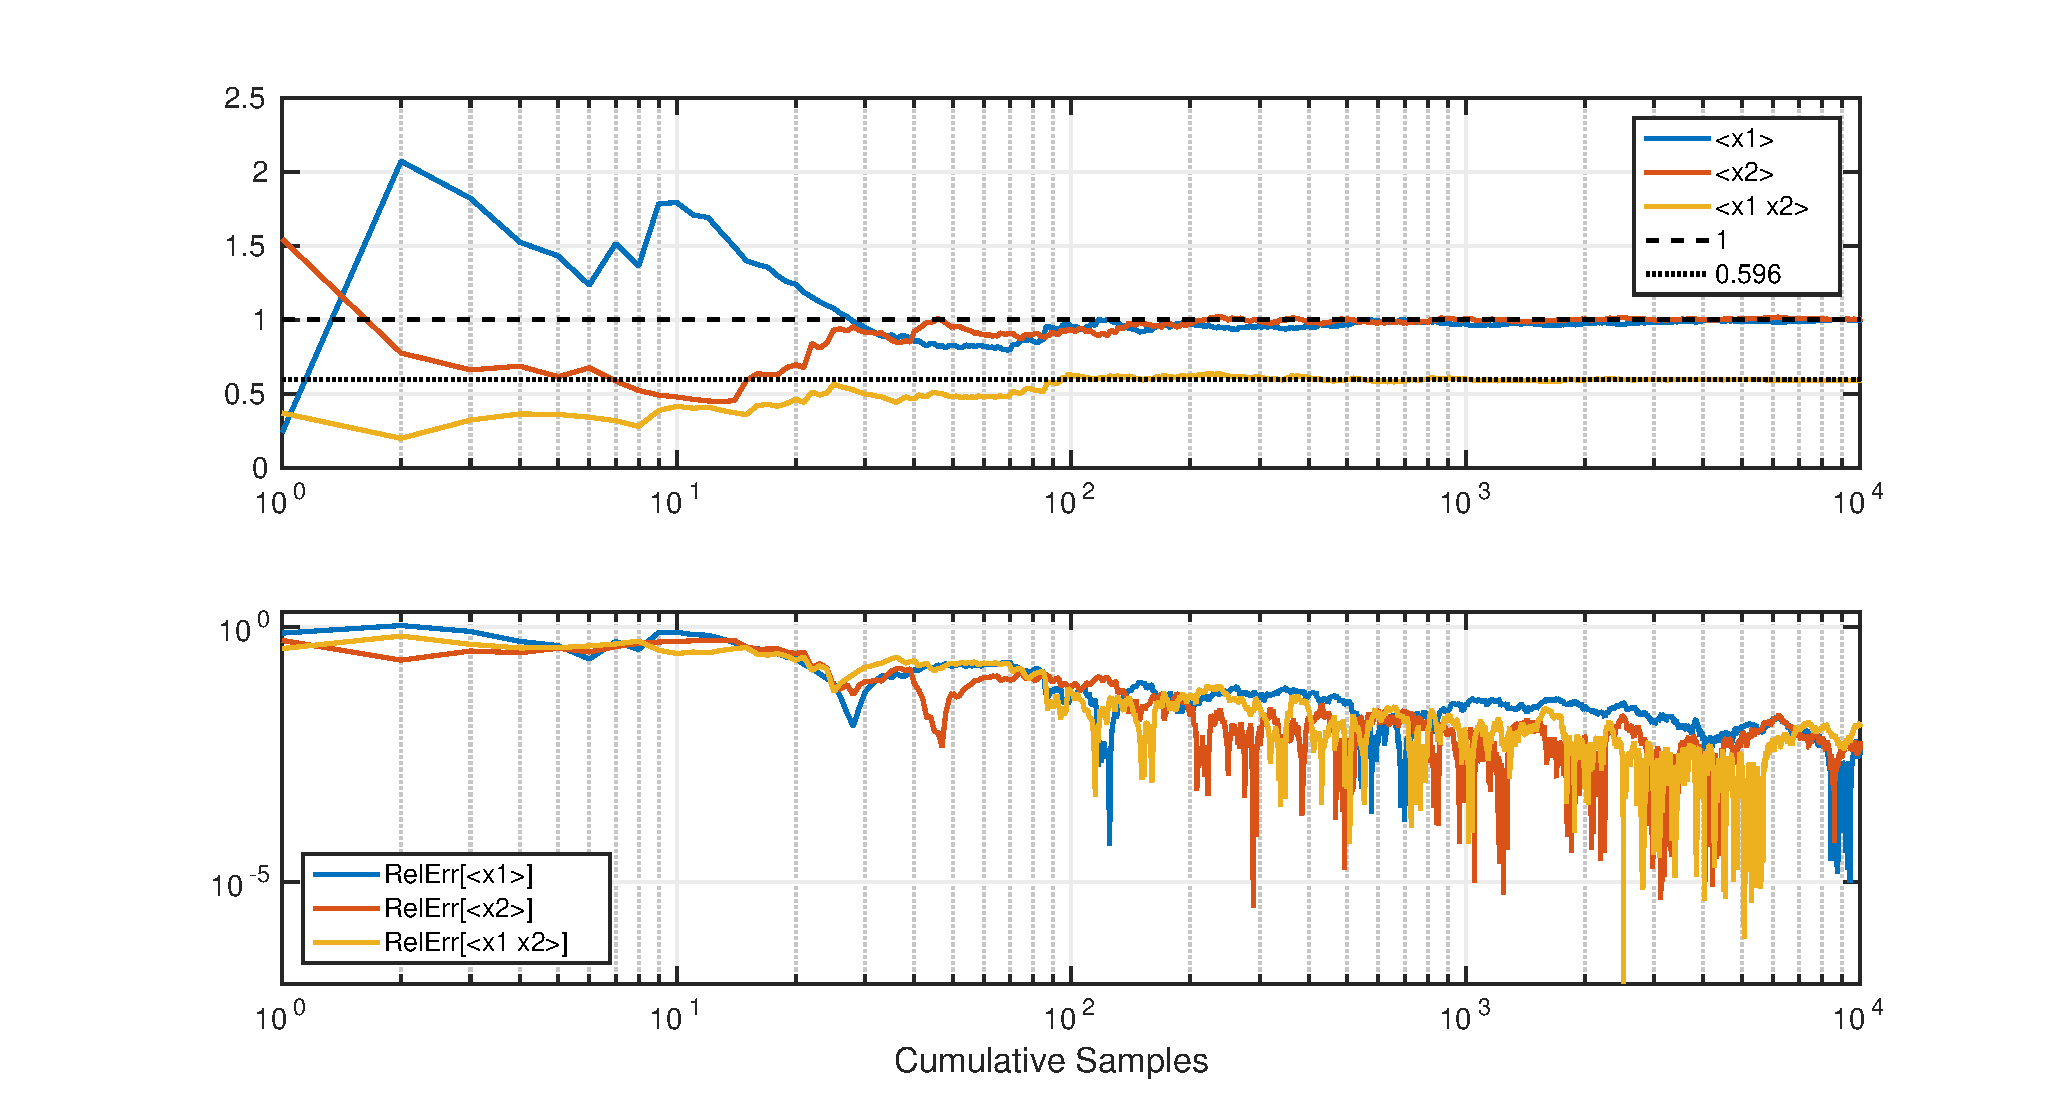
\includegraphics[width=\textwidth, trim={1in 0 1in 0}]{Prob1.eps}
\caption{Expectation values of various functions of $x_1$ and $x_2$, using the first $n$ cumulative samples. Analytical expectation values plotted to show convergence, as well as relative error.}
\label{fig:prob1}
\end{figure}

%%%%%%%%%%%%%%%%%%%%%%%%%%%%%%%%%%%%%%%%%%%%%%%%%
%%%%%%%%%%%%%%%%%%%%%%%%%%%%%%%%%%%%%%%%%%%%%%%%%
\section*{Problem 2} %%%%%%%%%%%%%%%%%%%%%%%%%%%%
%%%%%%%%%%%%%%%%%%%%%%%%%%%%%%%%%%%%%%%%%%%%%%%%%
%%%%%%%%%%%%%%%%%%%%%%%%%%%%%%%%%%%%%%%%%%%%%%%%%

This problem concerns a derivation from scratch of the Bayesian MAP estimate of a random variable $V$, assuming a Gaussian prior $V \sim N(V_0, \sigma_0^2)$. Further details are worked by hand on the attached sheets.

%%%%%%%%%%%%%%%%%%%%%%%%%%%%%%%%%%%%%%%%%%%%%%%%%
%%%%%%%%%%%%%%%%%%%%%%%%%%%%%%%%%%%%%%%%%%%%%%%%%
\section*{Problem 3} %%%%%%%%%%%%%%%%%%%%%%%%%%%%
%%%%%%%%%%%%%%%%%%%%%%%%%%%%%%%%%%%%%%%%%%%%%%%%%
%%%%%%%%%%%%%%%%%%%%%%%%%%%%%%%%%%%%%%%%%%%%%%%%%

The thermal coefficient $K$ of a 1D slab is characterized by a lognormal random process
\begin{equation*}
K(x,\omega) = \exp(G(x,\omega)), \qquad x \in (0,1),
\end{equation*}
where $G(x, \omega)$ is a Gaussian random process defined on $(0, 1)$. The mean and covariance functions of the Gaussian process $G(x, \omega)$ are
\begin{equation*}
\xpect{G(x)} = 1.0, \qquad x \in (0,1),
\end{equation*}
and
\begin{equation*}
C_{GG}(x_1,x_2) = \sigma^2 \exp \left( \frac{- | x_1-x_2 | }{\ell} \right), \qquad (x1,x2) \in (0,1) \times (0,1),
\end{equation*}
respectively. We would like to compute the statistics of the temperature field $u(x)$ by solving the governing steady-sate stochastic heat equation
\begin{align}
\pp{}{x} \left( K(x,\omega) \pp{u(x,\omega)}{x} \right) &= 1.0, \qquad x \in (0,1), \\
u(0,\omega) &= 0, \\
u(1,\omega) &= \theta(\omega),
\label{eq:pde}
\end{align}
where $\theta(\omega) \sim N(0,0.1)$ characterizes the uncertainty in the right boundary condition and is statistically independent from $K(x,\omega)$. Set $\sigma=2$ and $\ell=0.2$, and use the codes form Homework 1 to generate samples of $G_d(x,\omega)$ when only $d=10$ terms in the KL expansion of $G(x,\omega)$ are used.

We write a standard second-order central-difference implicit code to solve the PDE in \eqref{eq:pde} for fixed $\omega$, meaning that $K(x,\omega) \rightarrow K(x)$ and $\theta(\omega) \rightarrow \theta$. Next, we compute the mean $\xpect{u(x)}$ and variance $\var(u(x))$ of the solution using a Monte Carlo simulation, and verify that these statistics converge as the number of samples is increased. Finally, letting $u_\tmax = \max_x u(x)$, we compute the probability that the maximum temperature on the slab exceeds a certain threshold,
\begin{equation}
P \left( u_\tmax > \xpect{u_\tmax} + 3 \cdot \sqrt{\var(u_\tmax)} \right)
.
\label{eq:probability}
\end{equation}

Using the analytical eigensystem solution for the Karhunen-Loeve expansion, realizations of $G$, $K$, and $u$ are shown in \figref{fig:prob3a}. As the number of realizations $n$ is increased from 1 to $N=100,\!000$, the mean and variance converge to the functions presented in \figref{fig:prob3b}. Both boundary conditions are satisfied, since $u(0)=0$ is fixed and  $u(1) = \theta(\omega) \sim N(0,0.1)$ matches in both mean and variance plots. Finally, we see the probability converge to a value near 0.015 in \figref{fig:prob3c}. Though not shown in this figure, the final statistics pertaining to $u_\tmax$ obtained from 100,000 realizations are shown in Table \ref{tbl:probabilities}.

\begin{table}[h]
\centering
\begin{tabular}{ll}
\toprule
Quantity & Value \\
\midrule
$\xpect{u_\tmax}$ & 0.12571 \\
$\var(u_\tmax)$ & 0.03383 \\
$P(\cdot)$ & 1.553 \% \\
\bottomrule
\end{tabular}
\vspace{1em}
\caption{Relevant quantities in \eqref{eq:probability} computed from 100,000 realizations.}
\label{tbl:probabilities}
\end{table}

\begin{figure}[t]
\centering
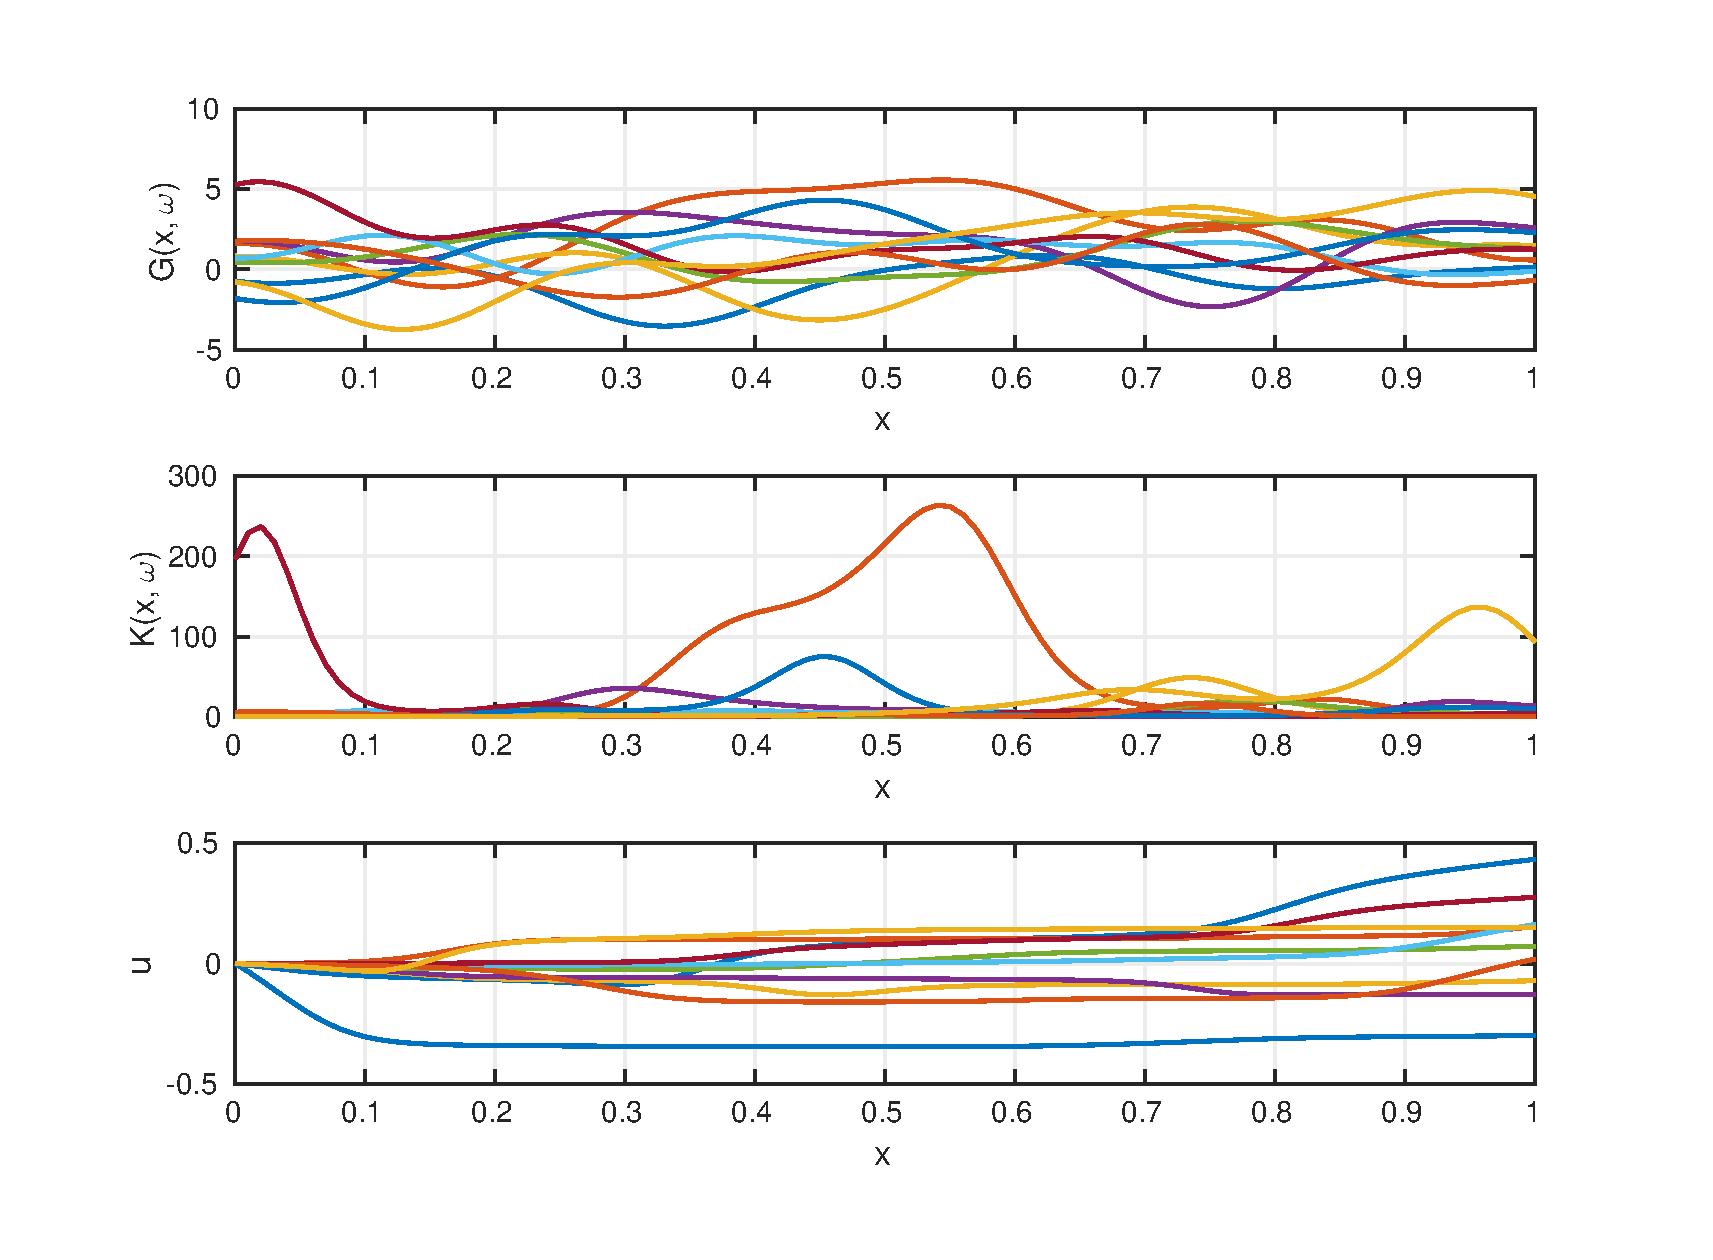
\includegraphics[width=0.84\textwidth, trim={1cm 0 1cm 0}]{Prob3_a.eps}
\caption{Ten realizations of $G$, $K$, and $u$.}
\label{fig:prob3a}
\end{figure}

\begin{figure}[b]
\centering
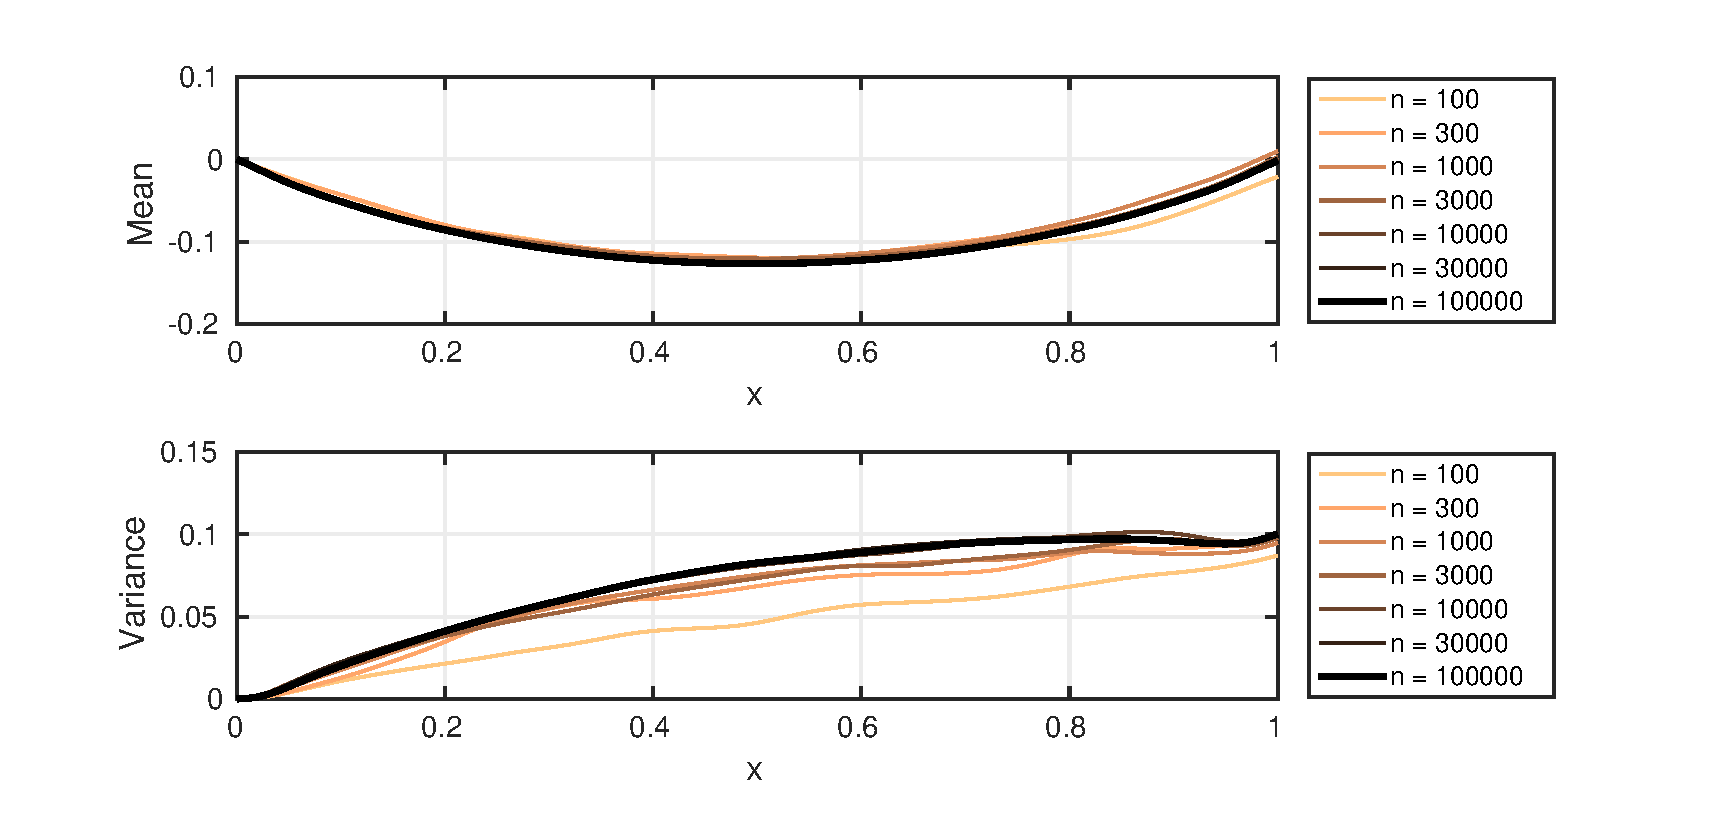
\includegraphics[width=0.9\textwidth, trim={1cm 0 1cm 0}]{Prob3_b.eps}
\caption{Convergence of the mean and variance of $u(x)$ as the number $n$ of realizations is increased.}
\label{fig:prob3b}
\end{figure}

\begin{figure}[t]
\centering
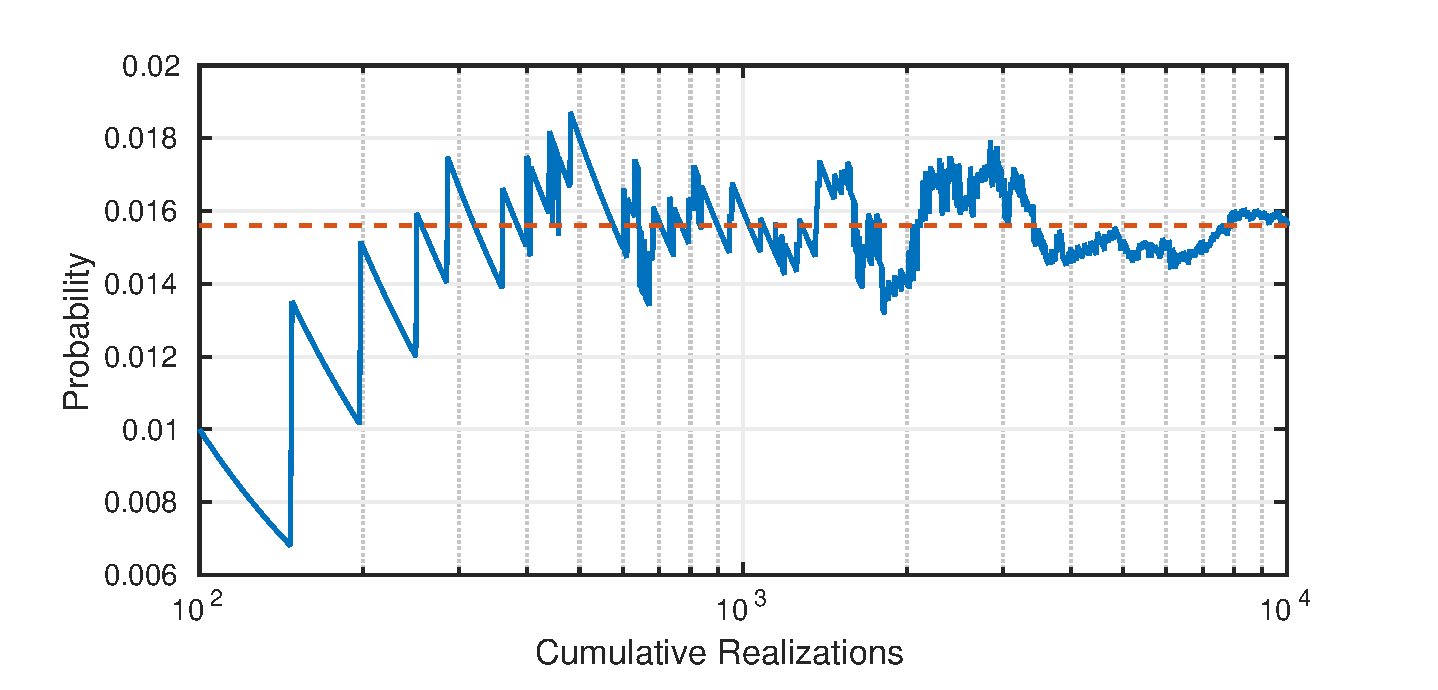
\includegraphics[width=0.9\textwidth, trim={1cm 0 1cm 0}]{Prob3_c.eps}
\vspace{1em}
\caption{Convergence in the probability \eqref{eq:probability} as more realizations are generated. Final statistics use $10^5$ realizations, but only up to $10^4$ are shown here.}
\label{fig:prob3c}
\end{figure}

%%
%% DOCUMENT END
%%
\end{document}
